\documentclass[aspectratio=169,11pt]{beamer}
\usetheme{Madrid}
\usepackage[T1]{fontenc}
\usepackage{lmodern}
\usepackage{amsmath,amssymb}
\usepackage{booktabs,tabularx,multicol}
\usepackage{pgfplots}
\pgfplotsset{compat=1.17}
\usepackage{tikz}
\usetikzlibrary{arrows.meta,positioning,shapes.geometric,fit,calc}

% ---------- colours (same palette as the Phase-1 / Phase-2 decks) ----------
\definecolor{navy}{HTML}{1F3A5F}
\definecolor{accent}{HTML}{2A78D6}
\definecolor{warm}{HTML}{EB6834}
\definecolor{aqua}{HTML}{1BAF7A}
\definecolor{gold}{HTML}{EDA100}
\definecolor{soft}{HTML}{EEF3FA}
\definecolor{ink}{HTML}{333333}
\setbeamercolor{structure}{fg=navy}
\setbeamercolor{palette primary}{bg=navy,fg=white}
\setbeamercolor{palette secondary}{bg=navy!85!black,fg=white}
\setbeamercolor{palette tertiary}{bg=navy!70!black,fg=white}
\setbeamercolor{frametitle}{bg=navy,fg=white}
\setbeamercolor{title}{bg=navy,fg=white}
\setbeamercolor{block title}{bg=accent,fg=white}
\setbeamercolor{block body}{bg=soft,fg=ink}
\setbeamercolor{block title alerted}{bg=warm,fg=white}
\setbeamercolor{block body alerted}{bg=warm!8,fg=ink}
\setbeamercolor{block title example}{bg=aqua,fg=white}
\setbeamercolor{block body example}{bg=aqua!8,fg=ink}
\setbeamertemplate{navigation symbols}{}
\setbeamertemplate{itemize items}[circle]
\setbeamertemplate{section in toc}[sections numbered]

\newcommand{\code}[1]{\texttt{\small #1}}
\newcommand{\bs}{\textbackslash}
\newcommand{\pb}[1]{\textbf{\textcolor{warm}{#1}}}   % problem tag
\newcommand{\mt}[1]{\textbf{\textcolor{aqua!80!black}{#1}}} % method tag
\newcommand{\yes}{\textcolor{aqua!80!black}{$\bullet$}}
\tikzset{
  box/.style={draw=navy,rounded corners=3pt,fill=soft,align=center,font=\scriptsize,minimum height=8mm,inner sep=3pt,text width=17mm},
  new/.style={box,fill=aqua!15,draw=aqua!70!black},
  arr/.style={-{Stealth[length=2mm]},thick,navy},
}

\title[CS-781: data audit and retraining plan]{Phase-1 Corpus Audit and Retraining Plan}
\subtitle{Current statistics, problems found, and the methods that address them}
\author[Manish Kumar]{Manish Kumar (251330604)}
\institute{CS-781, IIT Kanpur}
\date{11 October 2026}

\begin{document}

\begin{frame}
  \titlepage
\end{frame}

\begin{frame}{Outline}
  \begin{multicols}{2}
  \tableofcontents
  \end{multicols}
\end{frame}

% =====================================================================
\section{Current statistics}

\begin{frame}{Phase-1 pretraining corpus as built today}
  \begin{columns}[T]
    \begin{column}{0.58\textwidth}
      \footnotesize
      \begin{tabular}{lrrrr}
        \toprule
        Source & Train docs & Train words & Tokens & Tok/word \\
        \midrule
        Acts           &   2{,}425 & 14.8M & 18.7M & 1.26 \\
        Supreme Court  &  12{,}163 & 44.4M & 53.8M & 1.21 \\
        High Courts    & 120{,}529 & 51.9M & 66.2M & 1.28 \\
        Tribunals      &  20{,}041 & 37.0M & 48.8M & 1.32 \\
        \midrule
        \textbf{Total} & \textbf{155{,}158} & \textbf{148.2M} & \textbf{187.5M} & 1.27 \\
        \bottomrule
      \end{tabular}

      \vspace{2mm}
      Validation: 3{,}764 documents, 5.0M tokens.\\
      Mix achieved: Acts 10\%, SC 28.7\%, HC 35.3\%, Tribunals 26\%.
    \end{column}
    \begin{column}{0.40\textwidth}
      \footnotesize
      \begin{block}{Pipeline (\code{legal\_lm/data/corpus.py})}
        \begin{itemize}
          \item Stream each source file from the start.
          \item Keep a doc with probability 0.5.
          \item \code{clean\_text}: replace NUL, collapse whitespace.
          \item Drop docs under 50 words.
          \item 1\% of docs to validation, rest to train.
          \item Stop when the word budget is full.
        \end{itemize}
      \end{block}
    \end{column}
  \end{columns}
\end{frame}

\begin{frame}{Phase-1 models: validation loss was still falling}
  \begin{columns}[T]
    \begin{column}{0.55\textwidth}
      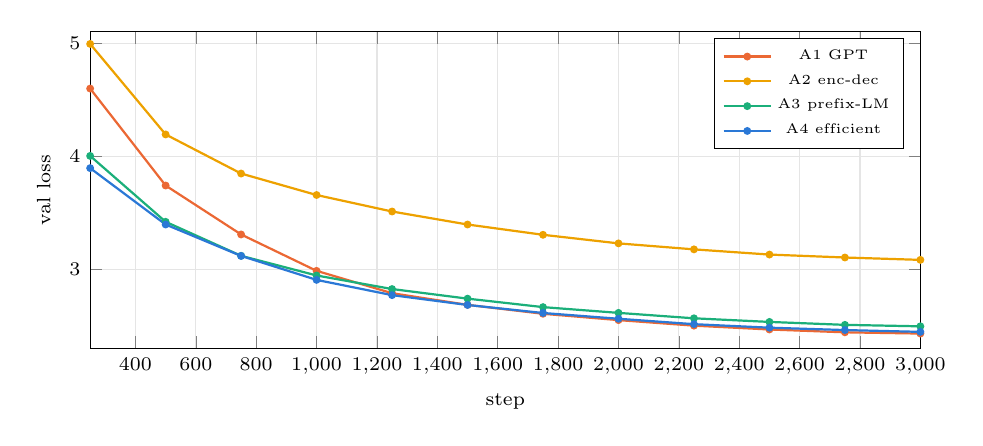
\begin{tikzpicture}
        \begin{axis}[width=\linewidth,height=5.6cm,xlabel={step},ylabel={val loss},
          xmin=250,xmax=3000,ymin=2.3,ymax=5.1,grid=major,grid style={gray!20},
          legend style={font=\tiny,at={(0.98,0.98)},anchor=north east},tick label style={font=\scriptsize},
          label style={font=\scriptsize}]
          \addplot[thick,color=warm,mark=*,mark size=1pt] coordinates {(250,4.598)(500,3.74)(750,3.307)(1000,2.985)(1250,2.787)(1500,2.684)(1750,2.605)(2000,2.549)(2250,2.5)(2500,2.466)(2750,2.441)(3000,2.43)};
          \addplot[thick,color=gold,mark=*,mark size=1pt] coordinates {(250,4.993)(500,4.192)(750,3.846)(1000,3.656)(1250,3.51)(1500,3.395)(1750,3.304)(2000,3.228)(2250,3.175)(2500,3.129)(2750,3.103)(3000,3.082)};
          \addplot[thick,color=aqua,mark=*,mark size=1pt] coordinates {(250,4.002)(500,3.419)(750,3.118)(1000,2.944)(1250,2.824)(1500,2.739)(1750,2.664)(2000,2.613)(2250,2.565)(2500,2.533)(2750,2.507)(3000,2.494)};
          \addplot[thick,color=accent,mark=*,mark size=1pt] coordinates {(250,3.894)(500,3.395)(750,3.117)(1000,2.905)(1250,2.77)(1500,2.683)(1750,2.612)(2000,2.561)(2250,2.513)(2500,2.482)(2750,2.461)(3000,2.445)};
          \legend{A1 GPT,A2 enc-dec,A3 prefix-LM,A4 efficient}
        \end{axis}
      \end{tikzpicture}
    \end{column}
    \begin{column}{0.43\textwidth}
      \footnotesize
      \begin{tabular}{lrr}
        \toprule
        Model & Params & Val ppl \\
        \midrule
        A1 GPT        & 82.1M & \textbf{11.36} \\
        A2 enc-dec    & 89.4M & 21.79 \\
        A3 prefix-LM  & 81.3M & 12.11 \\
        A4 efficient  & 87.5M & 11.53 \\
        \bottomrule
      \end{tabular}

      \vspace{2mm}
      \begin{itemize}
        \item 3000 steps, 196.6M tokens, about 0.75 GPU-hours for A4.
        \item Curves flatten because the cosine LR ends, not because the models converged.
        \item Mean GPU utilisation during A4 training: 28\%.
      \end{itemize}
    \end{column}
  \end{columns}
\end{frame}

\begin{frame}{Phase 2 (Legal NER) on top of these models}
  \begin{columns}[T]
    \begin{column}{0.50\textwidth}
      \footnotesize
      \begin{block}{Dev strict macro-F1, mean $\pm$ std over 3 dev splits}
        \begin{tabular}{lcc}
          \toprule
          Run & No post-proc. & Best post-proc. \\
          \midrule
          E2 (A4 + LoRMA)  & 0.488 $\pm$ .007 & \textbf{0.518 $\pm$ .016} \\
          E2 inv-sqrt, r32 & \textbf{0.497 $\pm$ .012} & 0.508 $\pm$ .013 \\
          A4 + LoRA        & 0.490 $\pm$ .018 & 0.517 $\pm$ .043 \\
          \bottomrule
        \end{tabular}
      \end{block}
      \begin{itemize}
        \item Tokenisation is not the bottleneck: oracle macro-F1 is 0.9945.
        \item Learning curve: 15 docs 0.339, 30 docs 0.448, 60 docs 0.49.
      \end{itemize}
    \end{column}
    \begin{column}{0.46\textwidth}
      \footnotesize
      \begin{block}{Per-label F1 (A4 + LoRA, dev split 0)}
        \begin{tabular}{lr@{\hspace{6mm}}lr}
          \toprule
          \multicolumn{2}{c}{Local pattern} & \multicolumn{2}{c}{Role in document} \\
          \midrule
          DATE   & 0.98 & APP  & \textcolor{warm}{0.10} \\
          STAT   & 0.84 & RESP & \textcolor{warm}{0.08} \\
          COURT  & 0.80 & AUTH & \textcolor{warm}{0.23} \\
          CASENO & 0.64 & WIT  & \textcolor{warm}{0.25} \\
          \bottomrule
        \end{tabular}
      \end{block}
      Span-only F1 about 0.60 against strict 0.50: about 10 points are lost to the right span with the wrong label.
    \end{column}
  \end{columns}
\end{frame}

% =====================================================================
\section{Problems identified}

\begin{frame}{Problems at a glance}
  \footnotesize
  \begin{tabularx}{\textwidth}{clXl}
    \toprule
    & Problem & Evidence & Severity \\
    \midrule
    \pb{A} & Under-trained base model & 187.5M of $>$4.5B tokens; about 9$\times$ below 20 tokens/parameter; val loss still falling & High \\
    \pb{B} & Validation leaks into train & 29 val docs are exact train copies; $\ge$52/500 val docs share $>$50\% of 13-grams with train & High \\
    \pb{C} & No deduplication & 1{,}090 exact duplicates; 1{,}176 extra copies of the same 300-char prefix & Medium \\
    \pb{D} & OCR word stutter & 566 docs, about 2.4M words (1.6\% of the corpus) & Medium \\
    \pb{E} & Encoding and markup noise & About 70 docs with U+FFFD; RTF control words; 513 Acts docs with long dot/dash runs & Low \\
    \pb{F} & Short template orders dominate HC & 32\% of HC docs under 200 words; HC median 291 words & Mixed \\
    \pb{G} & Token budget missed & Estimated 1.35 tokens/word, measured 1.27 & Low \\
    \pb{H} & Head-of-file sampling & Each file is read from the start until its budget fills & Unverified \\
    \pb{I} & Long-range NER labels & APP/RESP depend on a header thousands of tokens away; window 512, A4 attention 256 & High (Phase 2) \\
    \bottomrule
  \end{tabularx}
\end{frame}

\begin{frame}{\pb{A}\,\, The base model saw too little text}
  \begin{columns}[T]
    \begin{column}{0.55\textwidth}
      \footnotesize
      \begin{itemize}
        \item The corpus offers more than 4.5B tokens; we used 187.5M (about 4\%).
        \item Rule of thumb of about 20 tokens per parameter gives about 1.7B tokens for an 87M model.
        \item Val loss of A4 dropped 0.037 over the last 500 steps while the LR was already near its minimum.
        \item The 200M figure was the course starter value, not a tuned choice.
      \end{itemize}
    \end{column}
    \begin{column}{0.42\textwidth}
      \begin{alertblock}{Consequence}
        \footnotesize
        Every later phase inherits a weak backbone. In Phase 2 no adaptation method (full, partial, LoRA, LoRMA, adapters, KD) pushed past about 0.50 macro-F1 without post-processing.
      \end{alertblock}
    \end{column}
  \end{columns}
\end{frame}

\begin{frame}{\pb{B}\,\, \pb{C}\,\, Leakage and duplicates}
  \begin{columns}[T]
    \begin{column}{0.50\textwidth}
      \footnotesize
      \begin{block}{Validation leakage}
        \begin{itemize}
          \item The split is drawn per document \emph{before} any duplicate check.
          \item 29 val documents also appear verbatim in train.
          \item 52 of 500 sampled val docs share more than half their 13-grams with only 30k of the 155k train docs: a lower bound.
          \item Phase-1 perplexities are therefore optimistic and checkpoint selection is biased.
        \end{itemize}
      \end{block}
    \end{column}
    \begin{column}{0.46\textwidth}
      \footnotesize
      \begin{block}{Duplicates inside train}
        \begin{itemize}
          \item 1{,}090 exact duplicates (0.7\%).
          \item 1{,}176 extra copies share the first 300 characters.
          \item Most common prefix appears 28 times:\\
            \textit{``GPN-J-332-ARHCB-8\_94-13,10,500-ALA4. SPL.H.C.A.S.C.D. 79e. FARAD FARAD FARAD CONTINUATION SHEET NO.\ldots''}
        \end{itemize}
      \end{block}
    \end{column}
  \end{columns}
\end{frame}

\begin{frame}{\pb{D}\,\, \pb{E}\,\, Noisy text that survives cleaning}
  \footnotesize
  \begin{block}{\pb{D} OCR stutter (Bombay HC scans, 566 docs)}
    \textit{``IN IN THE HIGH COURT OF JUDICAUTRE AT BOMBAY \ldots\ CIVIL CIVIL WRIT WRIT WRIT PETITION NO.\ 7880 OF 2004 Madanlal Veerchand Parekh Parekh Parekh Petitioner Petitioner Petitioner \ldots\ CORAM CORAM CORAM''}\\[1mm]
    Teaches repetition, and corrupts exactly the party, counsel and coram region that NER relies on.
  \end{block}
  \begin{columns}[T]
    \begin{column}{0.50\textwidth}
      \begin{block}{\pb{E} RTF and encoding residue (tribunals)}
        \texttt{\bs tab ( L.K. JOSHI )\bs par \bs pard\bs nowidctlpar\bs sl480 \ldots\ \bs lquote sd\bs rquote\bs f1\bs par \} }\textcolor{warm}{\textbf{?}}\\[1mm]
        About 70 docs contain the U+FFFD replacement character.
      \end{block}
    \end{column}
    \begin{column}{0.46\textwidth}
      \begin{block}{\pb{E} Blank-form filler (Acts)}
        \textit{``Signature .................................... Date ..................................''}\\[1mm]
        513 Acts docs (21\%) contain runs of 20+ dots, dashes or underscores.
      \end{block}
    \end{column}
  \end{columns}
\end{frame}

\begin{frame}{\pb{F}\,\, \pb{G}\,\, \pb{H}\,\, Mixing and sampling}
  \begin{columns}[T]
    \begin{column}{0.36\textwidth}
      \footnotesize
      \begin{block}{\pb{F} Template orders}
        \begin{tabular}{lrr}
          \toprule
          Source & Median & p10 \\
          \midrule
          Acts   & 2{,}535 & 410 \\
          SC     & 2{,}289 & 432 \\
          HC     & \textcolor{warm}{291} & \textcolor{warm}{95} \\
          Trib.  & 971 & 231 \\
          \bottomrule
        \end{tabular}\\[1mm]
        Words per document. 38{,}426 HC docs are under 200 words, mostly one-page orders with the same header template.
      \end{block}
    \end{column}
    \begin{column}{0.30\textwidth}
      \footnotesize
      \begin{block}{\pb{G} Budget estimate}
        Budgets are counted in words with 1.35 tokens/word. The measured value is 1.21--1.32, so training got 187.5M instead of 200M tokens.
      \end{block}
    \end{column}
    \begin{column}{0.30\textwidth}
      \footnotesize
      \begin{block}{\pb{H} Head-of-file sampling}
        Each file is streamed from its first record and reading stops once the budget fills. If files are ordered by court or year, the sample is skewed. \emph{Not yet verified.}
      \end{block}
    \end{column}
  \end{columns}
\end{frame}

\begin{frame}{\pb{I}\,\, Role labels need document-level context}
  \begin{columns}[T]
    \begin{column}{0.52\textwidth}
      \footnotesize
      \begin{itemize}
        \item Roles are declared once in the header: \textit{``JAGE RAM \& ORS.\ ..Appellants Versus STATE OF HARYANA ..Respondent''}.
        \item The same names recur thousands of tokens later, where the label must be inferred.
        \item Phase-2 documents: median about 4{,}500 words, max about 20{,}000.
        \item The tagger sees 512-token windows; A4 attention reaches 256 tokens.
        \item Evidence: label propagation across the document was the only reliable gain in the sweep (+0.02 to +0.03).
      \end{itemize}
    \end{column}
    \begin{column}{0.44\textwidth}
      \begin{alertblock}{Also: annotation ceiling}
        \footnotesize
        In the first training document the header party ``JAGE RAM \& ORS.'' is not tagged APP, while a later mention is. Some APP/RESP errors are against incomplete gold, which caps achievable F1.
      \end{alertblock}
    \end{column}
  \end{columns}
\end{frame}

% =====================================================================
\section{Methods}

\begin{frame}{Methods we will apply}
  \scriptsize\renewcommand{\arraystretch}{0.95}
  \begin{tabularx}{\textwidth}{clX}
    \toprule
    & Method & What it does \\
    \midrule
    \mt{M1} & Exact and near-duplicate removal & Hash of normalised text, then MinHash-LSH on word shingles; keep one doc per cluster \\
    \mt{M2} & Leak-free split and overlap check & Split by duplicate cluster after M1; assert zero exact and near-duplicate overlap between val and train \\
    \mt{M3} & OCR stutter repair and filter & Collapse ``w w w'' to ``w''; drop docs whose stutter ratio stays high \\
    \mt{M4} & Character and markup normalisation & Unicode NFKC; strip RTF control words; drop docs with U+FFFD; squeeze long dot/dash runs \\
    \mt{M5} & Quality filters and source caps & Per-source minimum length; letter-ratio filter; cap the share of short HC template orders \\
    \mt{M6} & Measured token budget & Measure tokens per word per source with the actual tokenizer; budget in tokens \\
    \mt{M7} & Whole-file random sampling & Sample uniformly across each file instead of reading from its start \\
    \mt{M8} & Continued pretraining at scale & Resume A4 (and A3) on 1--2B cleaned tokens with a re-warmed LR; raise GPU utilisation \\
    \mt{M9} & Document-context NER & Header-role propagation used in training as well as inference; longer effective context \\
    \mt{M10} & Audit as a regression test & Re-run \code{audit.py} on every new corpus; every problem count must reach its target \\
    \bottomrule
  \end{tabularx}
\end{frame}

\begin{frame}{Which method tackles which problem}
  \centering
  \small
  \begin{tabular}{l*{10}{c}}
    \toprule
    & \mt{M1} & \mt{M2} & \mt{M3} & \mt{M4} & \mt{M5} & \mt{M6} & \mt{M7} & \mt{M8} & \mt{M9} & \mt{M10} \\
    \midrule
    \pb{A} Under-trained base     &      &      &      &      &      & \yes & \yes & \yes &      &      \\
    \pb{B} Val leakage            & \yes & \yes &      &      &      &      &      &      &      & \yes \\
    \pb{C} Duplicates             & \yes &      &      &      &      &      &      &      &      & \yes \\
    \pb{D} OCR stutter            &      &      & \yes &      & \yes &      &      &      &      & \yes \\
    \pb{E} Encoding/markup noise  &      &      &      & \yes & \yes &      &      &      &      & \yes \\
    \pb{F} Short template orders  & \yes &      &      &      & \yes &      &      &      &      & \yes \\
    \pb{G} Token budget missed    &      &      &      &      &      & \yes &      &      &      &      \\
    \pb{H} Head-of-file sampling  &      &      &      &      &      &      & \yes &      &      & \yes \\
    \pb{I} Long-range NER labels  &      &      &      &      &      &      &      & \yes & \yes &      \\
    \bottomrule
  \end{tabular}
\end{frame}

\begin{frame}{New data pipeline}
  \centering
  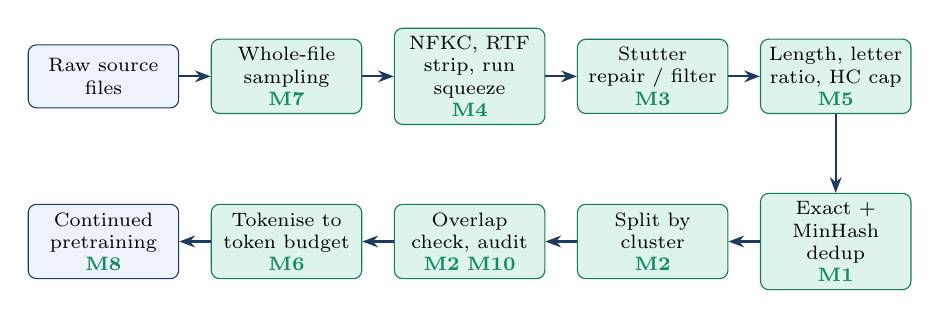
\begin{tikzpicture}[node distance=4mm]
    \node[box] (raw) {Raw source files};
    \node[new,right=of raw] (samp) {Whole-file sampling\\\mt{M7}};
    \node[new,right=of samp] (norm) {NFKC, RTF strip, run squeeze\\\mt{M4}};
    \node[new,right=of norm] (ocr) {Stutter repair / filter\\\mt{M3}};
    \node[new,right=of ocr] (qual) {Length, letter ratio, HC cap\\\mt{M5}};
    \node[new,below=10mm of qual] (dedup) {Exact + MinHash dedup\\\mt{M1}};
    \node[new,left=of dedup] (split) {Split by cluster\\\mt{M2}};
    \node[new,left=of split] (check) {Overlap check, audit\\\mt{M2} \mt{M10}};
    \node[new,left=of check] (tok) {Tokenise to token budget\\\mt{M6}};
    \node[box,left=of tok] (train) {Continued pretraining\\\mt{M8}};
    \draw[arr] (raw)--(samp); \draw[arr] (samp)--(norm); \draw[arr] (norm)--(ocr); \draw[arr] (ocr)--(qual);
    \draw[arr] (qual)--(dedup); \draw[arr] (dedup)--(split); \draw[arr] (split)--(check); \draw[arr] (check)--(tok); \draw[arr] (tok)--(train);
  \end{tikzpicture}

  \vspace{6mm}
  \footnotesize
  Green steps are new. Today's pipeline only has the grey boxes plus NUL removal, whitespace collapse and a 50-word minimum.
\end{frame}

\begin{frame}{\mt{M1}--\mt{M5}\,\, Cleaning methods in detail}
  \begin{columns}[T]
    \begin{column}{0.50\textwidth}
      \scriptsize
      \begin{block}{\mt{M1} \mt{M2} Deduplication and split}
        \begin{itemize}
          \item Exact: hash of lower-cased, whitespace-normalised text.
          \item Near: MinHash signatures over word shingles, LSH buckets, Jaccard threshold to be chosen on a labelled sample.
          \item Assign whole clusters to train or val, so no near-copy straddles the split.
          \item Check after splitting: 0 exact copies, 0 val docs above the overlap threshold.
        \end{itemize}
      \end{block}
      \begin{block}{\mt{M3} OCR stutter}
        \begin{itemize}
          \item Repair: replace a word repeated three times in a row with one copy.
          \item Filter: drop docs where repairs touch a large share of the words.
        \end{itemize}
      \end{block}
    \end{column}
    \begin{column}{0.46\textwidth}
      \scriptsize
      \begin{block}{\mt{M4} Characters and markup}
        \begin{itemize}
          \item Unicode NFKC normalisation.
          \item Strip RTF control words (\code{\bs par}, \code{\bs pard}, \code{\bs tab}, \code{\bs f1}, \ldots).
          \item Drop docs containing U+FFFD.
          \item Squeeze runs of dots, dashes, underscores to three characters.
        \end{itemize}
      \end{block}
      \begin{block}{\mt{M5} Quality and mixing}
        \begin{itemize}
          \item Per-source minimum length instead of one global 50 words.
          \item Drop docs with a low share of letters.
          \item Cap the token share of short HC orders; keep enough for header patterns.
        \end{itemize}
      \end{block}
    \end{column}
  \end{columns}
\end{frame}

\begin{frame}{\mt{M6}--\mt{M10}\,\, Scale, sampling, NER and checks}
  \begin{columns}[T]
    \begin{column}{0.50\textwidth}
      \scriptsize
      \begin{block}{\mt{M6} \mt{M7} Budget and sampling}
        \begin{itemize}
          \item Tokenise a sample per source and use the measured tokens/word.
          \item Count the budget in tokens at the tokenise step.
          \item Index record offsets, or use reservoir sampling, to sample evenly across each file.
        \end{itemize}
      \end{block}
      \begin{block}{\mt{M8} Continued pretraining}
        \begin{itemize}
          \item Resume from \code{runs/A4\_efficient/last.pt} (and A3).
          \item 1--2B cleaned tokens, LR re-warmed then decayed again.
          \item Raise throughput from 28\% GPU utilisation: larger micro-batch, \code{torch.compile}, more loader workers.
        \end{itemize}
      \end{block}
    \end{column}
    \begin{column}{0.46\textwidth}
      \scriptsize
      \begin{block}{\mt{M9} Document-context NER}
        \begin{itemize}
          \item Extract header roles (Appellant / Respondent / Petitioner lines).
          \item Apply label propagation during training, not only at inference.
          \item Larger windows where memory allows.
        \end{itemize}
      \end{block}
      \begin{block}{\mt{M10} Audit as a regression test}
        \begin{itemize}
          \item Same script as this audit, run on each new corpus.
          \item Fails the build if any count in the targets table is above its target.
        \end{itemize}
      \end{block}
    \end{column}
  \end{columns}
\end{frame}

% =====================================================================
\section{Experiment plan and success criteria}

\begin{frame}{Experiment plan: separate the effect of cleaning from scale}
  \footnotesize
  \begin{tabularx}{\textwidth}{lXll}
    \toprule
    Run & Change & Tokens & Isolates \\
    \midrule
    R0 & Current A4 checkpoint, re-evaluated on the new leak-free val set & 187.5M & Baseline \\
    R1 & A4 from scratch on cleaned data (\mt{M1}--\mt{M7}), same budget & 200M & Effect of cleaning \\
    R2 & R1 continued on more cleaned data (\mt{M8}) & 1--2B & Effect of scale \\
    R3 & R2 plus Phase-2 training texts in the mix (domain-adaptive) & R2 + small & Effect of in-domain text \\
    N1 & Phase-2 E2 recipe on R1 / R2 / R3 backbones & -- & Downstream gain \\
    N2 & N1 best backbone + document-context NER (\mt{M9}) & -- & Effect of \pb{I} fix \\
    \bottomrule
  \end{tabularx}

  \vspace{3mm}
  \begin{block}{Fair comparison}
    \footnotesize
    All runs, including R0, are scored on the same new leak-free validation set. Phase-2 numbers are mean $\pm$ std over dev splits 0, 1, 2, with and without post-processing.
  \end{block}
\end{frame}

\begin{frame}{Success criteria}
  \begin{columns}[T]
    \begin{column}{0.52\textwidth}
      \footnotesize
      \begin{block}{Corpus audit targets (\mt{M10})}
        \begin{tabular}{lrr}
          \toprule
          Check & Today & Target \\
          \midrule
          Val docs exactly in train   & 29     & 0 \\
          Val docs $>$50\% 13-gram overlap & $\ge$52/500 & 0 \\
          Exact duplicate train docs  & 1{,}090 & 0 \\
          Docs with heavy OCR stutter & 566    & 0 \\
          Docs with U+FFFD            & about 70 & 0 \\
          Train tokens vs budget      & 93.7\% & $\approx$100\% \\
          \bottomrule
        \end{tabular}
      \end{block}
    \end{column}
    \begin{column}{0.44\textwidth}
      \footnotesize
      \begin{block}{Model targets}
        \begin{itemize}
          \item R1 vs R0: lower val perplexity on the leak-free val set at equal tokens.
          \item R2 vs R1: val loss keeps falling with more tokens.
          \item N1 vs current E2: higher Phase-2 macro-F1 with no post-processing (today 0.488 $\pm$ .007).
          \item N2: APP and RESP F1 well above today's 0.10 / 0.08.
        \end{itemize}
      \end{block}
    \end{column}
  \end{columns}
\end{frame}

\begin{frame}{Summary}
  \begin{columns}[T]
    \begin{column}{0.48\textwidth}
      \footnotesize
      \begin{alertblock}{Problems}
        \begin{itemize}
          \item \pb{A} Base model trained on about 4\% of the corpus.
          \item \pb{B} \pb{C} Val leaks into train; duplicates kept.
          \item \pb{D} \pb{E} OCR stutter, RTF and encoding noise.
          \item \pb{F} \pb{G} \pb{H} Skewed mix, missed budget, head-of-file sampling.
          \item \pb{I} NER role labels need document context.
        \end{itemize}
      \end{alertblock}
    \end{column}
    \begin{column}{0.48\textwidth}
      \footnotesize
      \begin{exampleblock}{Methods}
        \begin{itemize}
          \item \mt{M1} \mt{M2} Deduplicate, then split by cluster.
          \item \mt{M3} \mt{M4} \mt{M5} Repair and filter noisy text.
          \item \mt{M6} \mt{M7} Measured budget, whole-file sampling.
          \item \mt{M8} Continue pretraining on 1--2B clean tokens.
          \item \mt{M9} Document-context NER.
          \item \mt{M10} Audit every new corpus.
        \end{itemize}
      \end{exampleblock}
    \end{column}
  \end{columns}
\end{frame}

\end{document}
